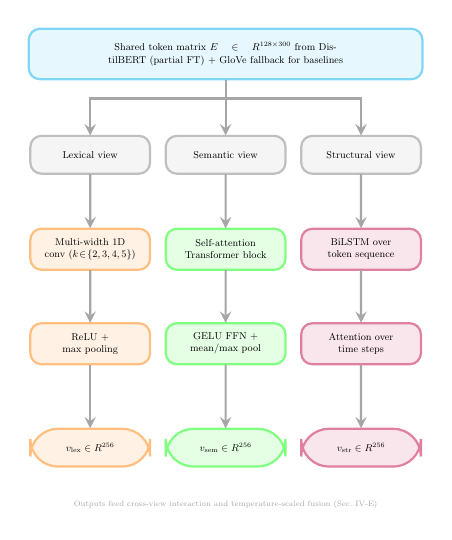
\begin{tikzpicture}[>=stealth, every node/.style={align=center},
                    scale=0.40, transform shape]

\tikzstyle{embedding}    = [rectangle, rounded corners=4pt, draw=cyan!50, fill=cyan!10,
                             thick, minimum width=12.5cm, minimum height=1.6cm,
                             text width=12.0cm, font=\small]
\tikzstyle{viewlabel}    = [rectangle, rounded corners=4pt, draw=gray!50, fill=gray!8,
                             thick, minimum width=3.8cm, minimum height=1.2cm, font=\small]
\tikzstyle{processorange}= [rectangle, rounded corners=4pt, draw=orange!50, fill=orange!10,
                             thick, minimum width=3.8cm, minimum height=1.3cm, font=\small]
\tikzstyle{processgreen} = [rectangle, rounded corners=4pt, draw=green!50, fill=green!10,
                             thick, minimum width=3.8cm, minimum height=1.3cm, font=\small]
\tikzstyle{processpurple}= [rectangle, rounded corners=4pt, draw=purple!50, fill=purple!10,
                             thick, minimum width=3.8cm, minimum height=1.3cm, font=\small]
\tikzstyle{outputorange} = [rectangle, rounded corners=10pt, draw=orange!50, fill=orange!10,
                             thick, minimum width=3.8cm, minimum height=1.2cm, font=\small]
\tikzstyle{outputgreen}  = [rectangle, rounded corners=10pt, draw=green!50, fill=green!10,
                             thick, minimum width=3.8cm, minimum height=1.2cm, font=\small]
\tikzstyle{outputpurple} = [rectangle, rounded corners=10pt, draw=purple!50, fill=purple!10,
                             thick, minimum width=3.8cm, minimum height=1.2cm, font=\small]
\tikzstyle{arrow}        = [->, >=stealth, thick, gray!70]
\tikzstyle{sectionlabel}  = [font=\bfseries\footnotesize, text=gray!80]

\def\colL{0}
\def\colM{4.3}
\def\colR{8.6}

\node[embedding] (embed) at (4.3, 0) {Shared token matrix $E \in \mathbb{R}^{128 \times 300}$ from DistilBERT (partial FT) + GloVe fallback for baselines};

\node[viewlabel]  (lexview) at (\colL, -3.2)  {Lexical view};
\node[viewlabel]  (semview) at (\colM, -3.2)  {Semantic view};
\node[viewlabel]  (strview) at (\colR, -3.2)  {Structural view};

\node[processorange] (conv)    at (\colL, -6.2) {Multi-width 1D\\conv ($k\!\in\!\{2,3,4,5\}$)};
\node[processorange] (maxpool) at (\colL, -9.2) {ReLU +\\max pooling};
\node[processgreen]  (selfattn)at (\colM, -6.2) {Self-attention\\Transformer block};
\node[processgreen]  (transenc)at (\colM, -9.2) {GELU FFN +\\mean/max pool};
\node[processpurple] (bilstm)  at (\colR, -6.2) {BiLSTM over\\token sequence};
\node[processpurple] (attnmech)at (\colR, -9.2) {Attention over\\time steps};

\node[outputorange]  (vlex) at (\colL, -12.5) {$v_{\mathrm{lex}} \in \mathbb{R}^{256}$};
\node[outputgreen]   (vsem) at (\colM, -12.5) {$v_{\mathrm{sem}} \in \mathbb{R}^{256}$};
\node[outputpurple]  (vstr) at (\colR, -12.5) {$v_{\mathrm{str}} \in \mathbb{R}^{256}$};

\draw[arrow] (embed.south) -- ++(0,-0.6) -| (lexview.north);
\draw[arrow] (embed.south) -- (semview.north);
\draw[arrow] (embed.south) -- ++(0,-0.6) -| (strview.north);

\draw[arrow] (lexview)  -- (conv);
\draw[arrow] (conv)     -- (maxpool);
\draw[arrow] (maxpool)  -- (vlex);

\draw[arrow] (semview)  -- (selfattn);
\draw[arrow] (selfattn) -- (transenc);
\draw[arrow] (transenc) -- (vsem);

\draw[arrow] (strview)  -- (bilstm);
\draw[arrow] (bilstm)   -- (attnmech);
\draw[arrow] (attnmech) -- (vstr);

\node[font=\scriptsize, text=gray!70] at (4.3, -14.3)
      {Outputs feed cross-view interaction and temperature-scaled fusion (Sec.~IV-E)};

\end{tikzpicture}
